\chapter{Audio-based methods}
In this section we will describe the possibilities of how to transform an audio file (in our case .wav) into representations suitable for song similarity calculations. This process consists of many steps and a lot of research has been done on all of them as illustrated in Section \ref{sec:audio_related_work}. \\
The reason we are focusing on audio in this thesis is the notion, that what people care about in a song is its sound. There are patterns in music that are pleasant to the human auditory system otherwise, music would not be so popular and we believe it is the sound wave that contains this information. It is difficult to define what exactly it is so we hope that with the use of unsupervised machine learning algorithms, we will be able to find these patterns and look for them in unseen songs as well. \\

Figure \ref{fig:audio_extraction} illustrates the steps of audio extraction. The blue part of the diagram describes the steps that are taken to acquire various basic music representations and are explained in Section \ref{sec:basic_music_representation_methods}. Each of these representations denoted can be given as input to a machine learning algorithm depicted in green from Section \ref{sec:audio_machine_learning} or deep learning algorithm from Section \ref{sec:audio_deep_learning} depicted in purple which both yield a final vector representation of the song. \\

\begin{figure}[h!]
    \centering
	\includegraphics[width=140mm]{./img/audio_feature_extraction_steps.png}
	\caption{A diagram displaying the steps taken in audio extraction. ML stands for machine learning and DL for deep learning.}
	\label{fig:audio_extraction}
\end{figure}

\section{Basic audio representation methods}\label{sec:basic_music_representation_methods}
 

\subsection{Raw waveform}
Sound is as vibration that spread through gas, liquid or solid as a wave of pressure. For humans, the sound we hear is has a frequency between 20Hz and 20kHz. Other sound waves are inaudible for humans. The most basic representation of an audio signal is a \textit{waveform}. It captures the variation of pressure over time. As we cannot store infinite data to capture the state of the wave in every moment, we need to establish a sample rate. The sample rate is the number of samples per second at which the pressure is recorded as amplitude. Common sample rates are 44 100 Hz and 22 050 Hz that capture oscillation up to 22 050 Hz and 11 025Hz.

\subsection{Spectrograms}
Raw waveform data have a lot of data points which make them spaciously demanding. Luckily, they also display strong regularities in their oscillations which gives us another, more compact possibility to represent audio signal. It encodes the signal as the strength of oscillations at different frequencies as opposed to amplitudes over time. Such an encoding is called a \textit{spectrum} when the sinusoids are used as prototypical oscillations.
The spectrum is obtained from the waveform by applying Discrete Fourier Transformation. The signal is then represented by oscillations of a few frequencies spanning the full signal. \\
However a problem with this approach is, that for longer recordings, many oscillations are present only over some limited time span or change frequency. To represent all the oscillations the \textbf{Short-Time Fourier Transformation} can be computed. It slices the audio into small often overlapping windows, computes their spectra and then puts them together in a chronological order. This spectra matrix is called the \textit{spectrogram} and for the song 'Someone Like You' by 'Adele' it has the shape of (2206, 7796). It can be visualized as a graph with frequency on one and time on the other axis. The intensity of a frequency is represented by color.

\begin{figure}[h!]
    \centering
	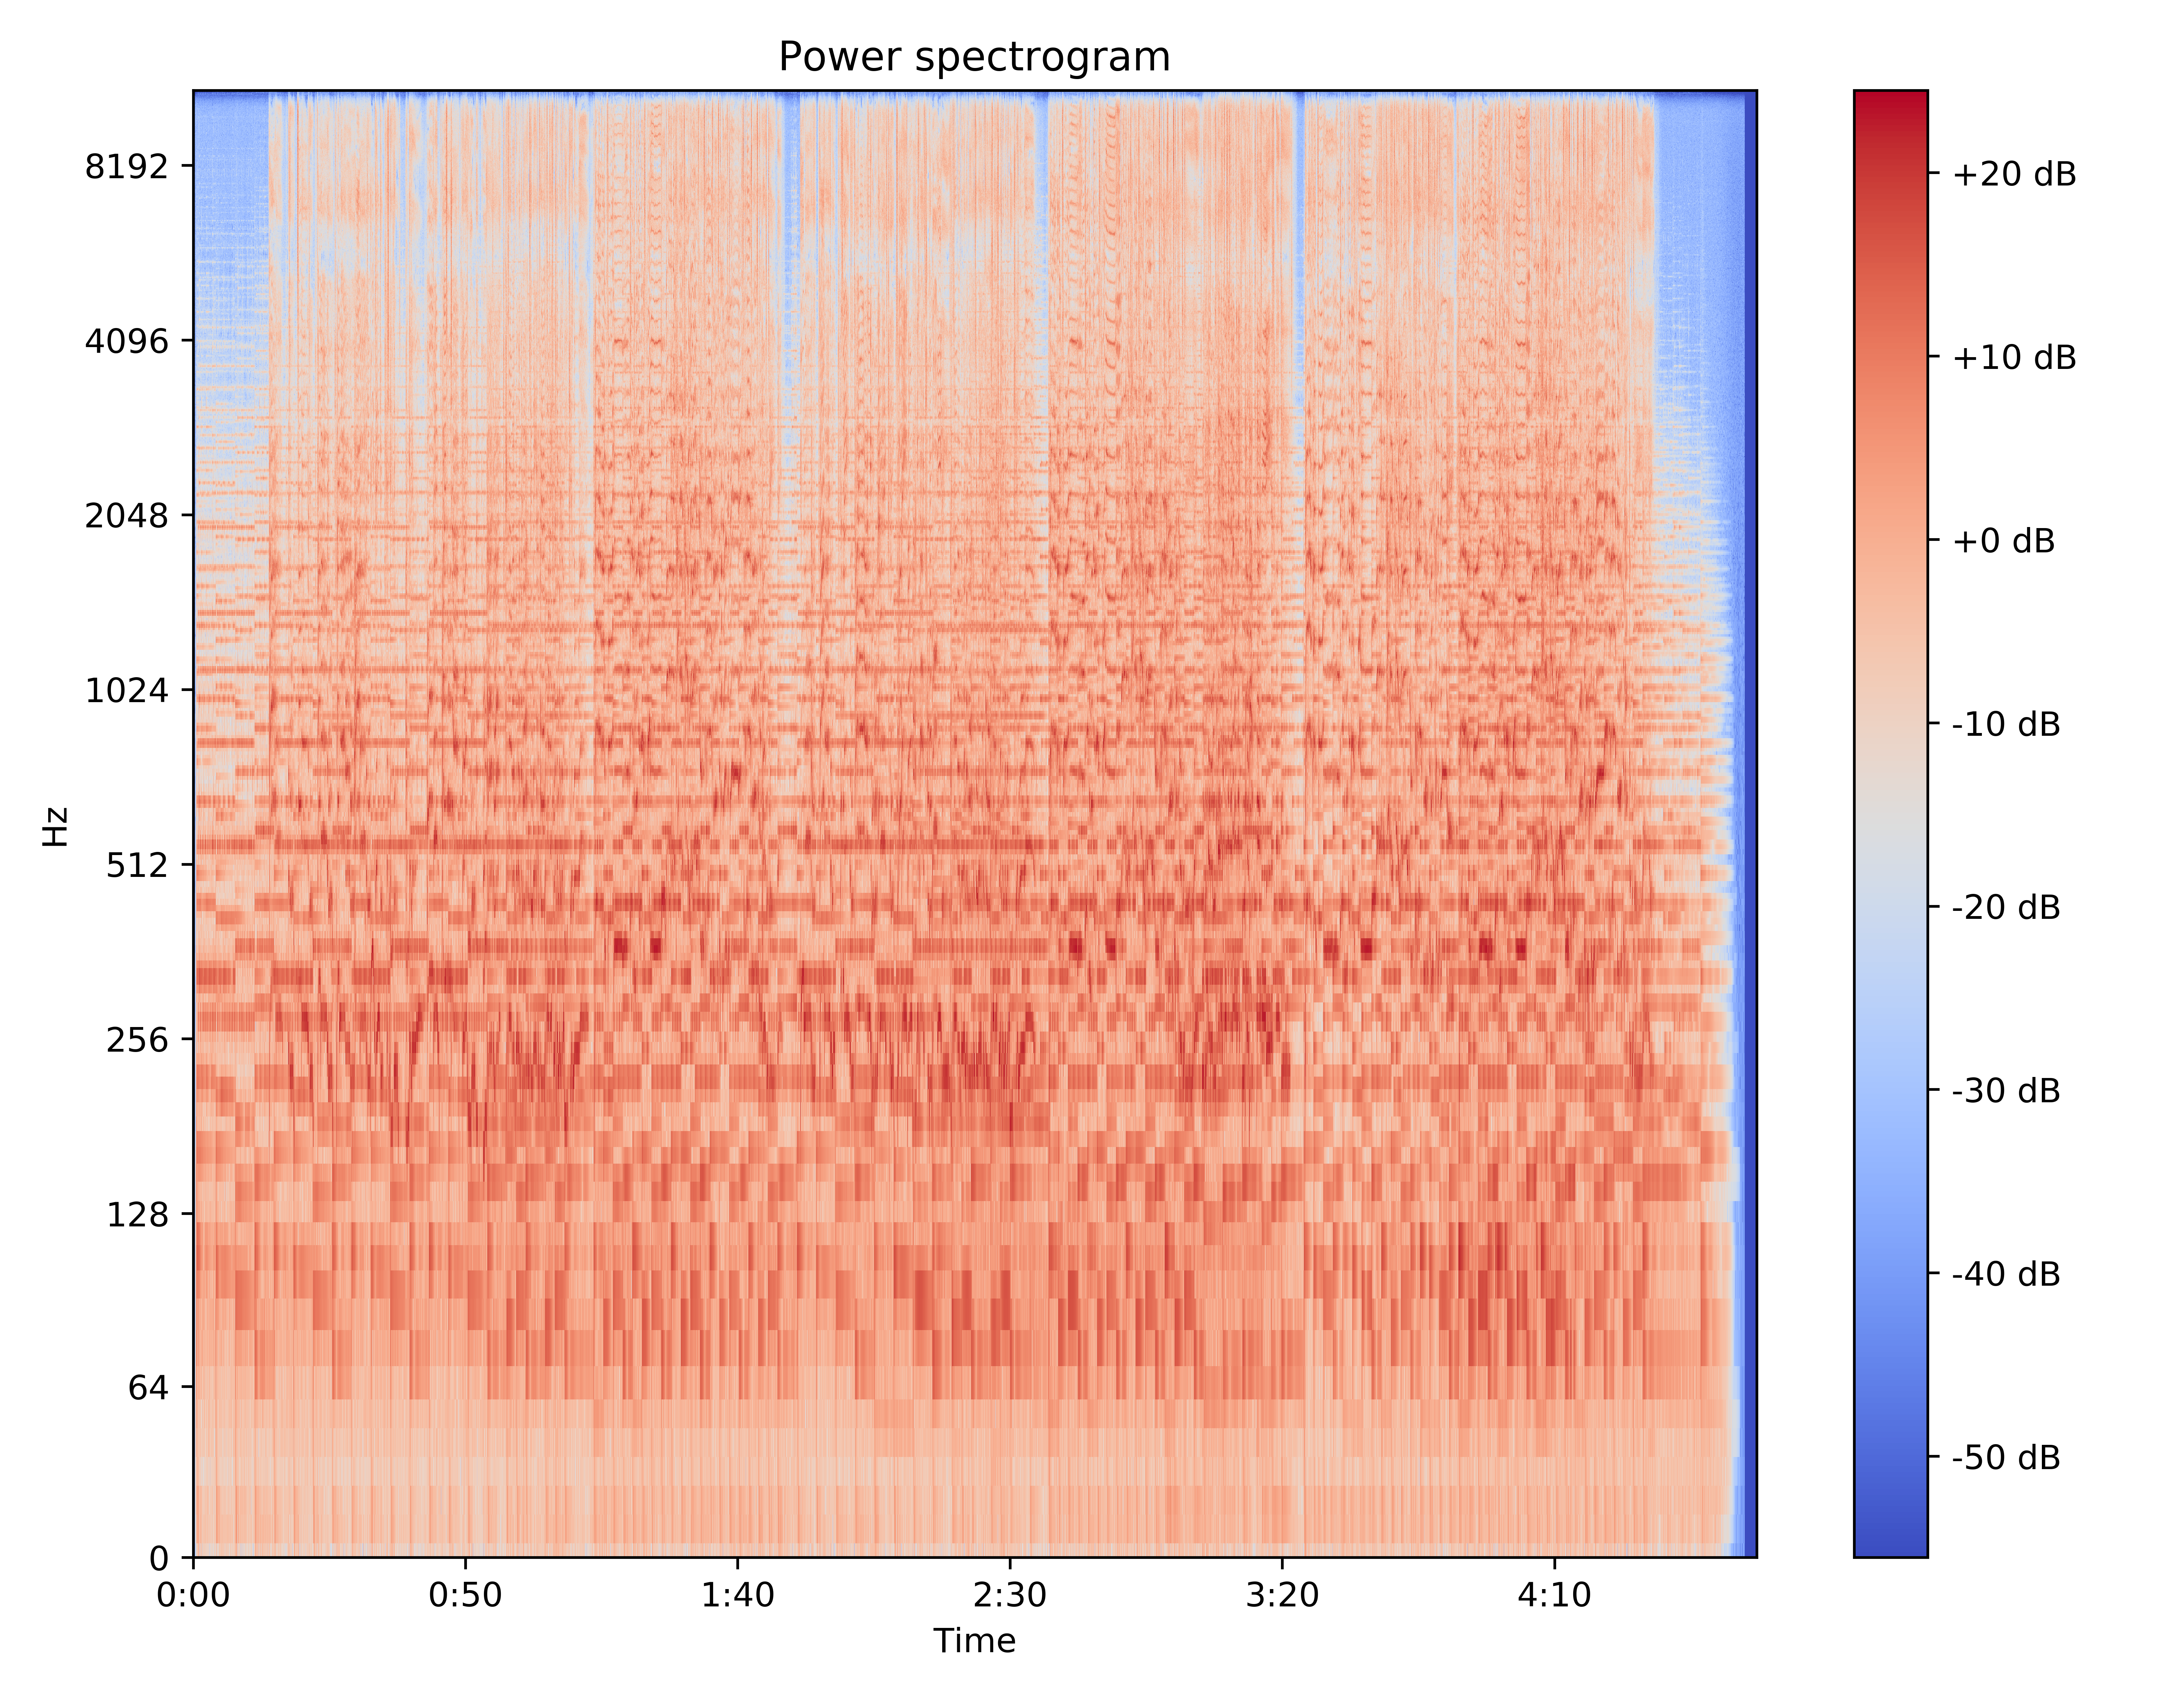
\includegraphics[width=140mm]{./img/spectrogram.png}
	\caption{Spectrogram of the song 'Someone Like You' by 'Adele'. The intensity of different frequencies over time is converted to decibels.}
	\label{fig:ilustrative_specrogram}
\end{figure}


\subsection{Mel Spectrograms}\label{ssec:mel_spectrograms_intro}
Mel-spectrograms are another approach to reducing the dimensionality of our data. However they are not mathematically based reductions of any kind of feature space. They are filtered spectrograms. Frequency bands are extracted by applying triangular \textit{Mel scale} filters to the power spectrum. The \textit{mel scale} after which this the spectrograms are called was named in 1937 in a study \cite{1937ASAJ....8..185S} by Volkmann and Newman. Since then it has been re-formulated multiple times, to mention for example \cite{mel_scale_fit} by Umesh at al. It is based on the human perception of pitch and loudness and allows us to convert from Hz to Mels which are more discriminatory at lower frequencies and less at higher frequencies - as is the human ear. As for the triangular filters, each of them has a response going from 1 to 0. They respond 1 at the center of some frequency and then their response decreases linearly to 0 towards to the place where they meet the neighbouring filters. When these filters are applied to a spectrogram, we get a mel-spectrogram. It is again a matrix with of a smaller shape (320, 7796) for 'Someone Like You' and it can also be visualized as can be seen in Figure \ref{fig:ilustrative_melspecrogram}.

\begin{figure}[h!]
    \centering
	\includegraphics[width=140mm]{./img/melspectrogram.png}
	\caption{Mel-spectrogram of the song 'Someone Like You' by 'Adele'. The intensity of different frequencies over time is converted to decibels.}
	\label{fig:ilustrative_melspecrogram}
\end{figure}

\subsection{Mel Frequency Ceptral Coefficients}
Mel-Frequency Ceptral Coefficients (MFCC) are another step further in extracting audio features. They are obtained by applying \textit{Discrete cosine transform} to mel-informed spectrograms. The DCT yield even more compressed representation of them. For the song 'Someone Like You' by 'Adele' which we used as an example for spectrograms as well as mel-spectrograms, it created a matrix of shape (128, 7796) which looks as Figure \ref{fig:ilustrative_mfccs} illustrates.

\begin{figure}[h!]
    \centering
	\includegraphics[width=140mm]{./img/mfccs.png}
	\caption{MFCCs of the song 'Someone Like You' by 'Adele'. The intensity of different frequencies over time is converted to decibels.}
	\label{fig:ilustrative_mfccs}
\end{figure}

\section{Simple audio representation methods}\label{sec:audio_machine_learning}

\subsection{PCA}
PCA is a common machine learning algorithm to reduce dimensionality of the feature space. It tries to keep only features with most variance and discards feature in which all the data points are highly correlated. The data space is transformed in such a way, that the first principal component (PC) has the largest possible variance, the second PC the second largest variance etc. \\
Mathematically it is a orthogonal linear transformation to a new coordinate system where the base vectors are the principal components. To achieve this, we first need to center the data around the origin. That is done by subtracting the mean of each variable from the data. After that a covariance matrix is computed with its eigenvalues and corresponding eigenvectors. After normalizing the eigenvectors, they can be interpreted as a new basis vector. This new basis transforms the covariance matrix so that it becomes diagonal. Each of the diagonal elements represents the variance of each axis. All the components without any reduction give us the whole information about the input data, only in a vector space with a different basis. Every component explains some portion of the data's variance. The variance can be calculated by dividing the eigenvalue corresponding to an eigenvector with the sum of all eigenvalues. The dimensionality reduction is dependant on how many components we want. If we want to visualize the input data in a 2D graph, we only have a space with the first two PCs. The reason to use this algorithm in our thesis would be mainly to reduce the length of the audio feature vectors. \\
The PCA assumes that there is linear correlation between features. If there is not, the PCA will not discover it and will loose a lot of information with the dimensionality reduction it performs.

\section{Deep audio representation methods}\label{sec:audio_deep_learning}

\subsection{Convolutional neural networks}
Convolutional neural networks are neural networks that have become extensively researched after AlexNet (a form of CNN) was demonstrated in 2012 and outperformed all other methods for visual classification \cite{Krizhevsky:2012:ICD:2999134.2999257}. As with other neural networks, CNN's biggest advantage is to emulate behavior of unknown non-linear functions. CNNs have the ability to map high-dimensional data into a space of finite categories (with hundreds or thousands of classes). They are mostly used in visual imagery tasks. \\
The idea behind convolutional neural networks is to use \textit{local filters} instead of creating fully connected layers. This has risen from the idea that in images, there are correlated compositions on short scale distances, rather than at large distances. For example when detecting a human face in an image with a tree in the background, the tree does not have much to say about the face, unlike the eyes or the nose by which the face can be identified and in a much greater proximity to each other. This is also the reason why in the CNN's architecture, the layers are not fully connected. \\
There are 4 main components that are generally be included in every CNN network. The \textit{Convolution layer},the \textit{ReLU}, the \textit{Maxpooling layer} and the \textit{Fully connected layer} that yields the output. To briefly describe these layers lets start with convolution. The convolutional layer helps to reduce the number of connections and weights. It consists of filters that can be learned. These only take a small number of nearby features into account at a time but extend through the whole input. Each of the filters crates a 2D activation map by computing the dot product of entries of the filter and the input. ReLU (rectified linear unit) is generally used to increase non linear properties of the decision function. It's function is $ f(x) = max(0,x) $ which is applied to the results of the convolution to speed up training --- compared to previously used functions for example sigmoid functions --- without affecting the receptive fields of the convolution layer. The pooling layer also reduces the number of parameters and helps prevent over-fitting. The most common function to implement is \textit{max pooling}. The features are partitioned into a set of non-overlapping rectangles (if input is 2D) and each of these rectangles  is represented by its maximal value. 
The final layer is usually a fully connected. Its neurons have connections to all activations of the previous layer and their activation is then computed as an affine transformation. 

\subsection{Deep belief networks}
Deep belief networks introduced by Hinton \cite{Hinton504} are multiple \textit{Restricted Boltzmann machines} greedily stacked on top of each other. RBMs are shallow two-layer neural nets created by Paul Smolensky in 1986 \cite{Smolensky1986InformationPI}. The first layes is called the visible layer, the second layer is called the hidden layer. The nodes of each layer communicate with with the previous and subsequent layer but there are no connections between nodes of the same layer. Each visible node takes a low level feature to be learned and multiplies it by some weight. The results for each feature of an input sample are then summed, bias is added and this is the result passed through and activation algorithm which produces an output for each hidden node. These outputs then can be redirected into another hidden layer instead of the output of the neural network. \\
RBMs also have the ability to reconstruct data without supervision. When the input makes it through both layers it then becomes input for the hidden layer and travels through the neural network in the opposite direction. The activations are multiplied by the same weights and passed to the visible layer where a new bias is added. The output of the visible layer is then compared to the initial input and the network adjusts weights so that it minimizes the difference between the input and the output.

\subsection{Recurrent neural networks}
Recurrent neural networks have one major difference compared to other neural networks. They include feedback loops in their structure which allows them to exhibit dynamic behaviour and makes them useful for processing sequential data. RNNs have a hidden state that is determined by previous states and is updated with every subsequent step. There are many variants of RNNs such as \textit{Fully recurrent, Long short-term memory introduced by Hochreiter and Schmidhuber in \cite{doi:10.1162/neco.1997.9.8.1735}, Gated recurent units first described in \cite{cho-etal-2014-learning}, or Bi-directional invented by Schuster and Paliwal in \cite{Schuster1997BidirectionalRN}}. \\
Recurrent neural networks are used for working with sequential data for example in speech recognition \cite{DBLP:journals/corr/abs-1303-5778} or time-series anomaly detection \cite{inproceedings_RNN_anomaly_detection}.


\subsection{Autoencoders}
Autoencoders are not tied to one type of neural network. They can be build from recurrent layers, convolutional layers or using a simple Multi-layer Perceptron. The autoencoder has two parts the encoder and the decoder. It is trained in an unsupervised manner. The encoder takes the input data and reduces it's dimensions. The decoder does not know, what the data looked like before the encoder processed it and tries to recreate it's original version. The idea is, that over time, the encoder learns how to shrink the data with retaining as much information as possible for the decoder so it is able to recreate the original form as accurately as possible. 

\section{Related work}\label{sec:audio_related_work}
For the signal representation, there is obviously the possibility to use raw audio data as input for the machine learning algorithm. This however is a quite uncommon approach and when tested recently in tag prediction \cite{6854950} it had worse results than the standard spectrogram. Multiple studies and experiments have been done using spectrograms as representation for classification tasks as for example \cite{wang2014improving} or to for unsupervised learning \cite{van2013deep}, \cite{Ramakrishnan2017song2V}, \cite{NIPS2009_3674}, which is what also our area of interest. \\
In these studies the inputs were fed into various neural network. The output of those was then evaluated and compared to trying to classify music or simply estimate music similarity with using similarity measures directly on spectrograms. We are going to do the same thing in this thesis.

\section{Conclusion and implementation choices}

\subsection{Basic audio representation choices}
At first when developing the web application we had the hope of using at least some of the raw data representation, to build some sort of base-line model. However, this turned out to be quite difficult as the vectors from spectrograms, mel-spectrograms and mfccs have tens sometimes even hundreds of thousands of features. Therefore, although we implemented and evaluated recommendations based on mel spectrograms and mfccs, to implement them turned out to be too time consuming to be included in the proposed web application. The specific reasons are described in more detail in Chapter \ref{chap:experiments}. For the application, only transformed mel-spectrograms and MFCCS were selected as they allow us to significantly reduce the dimensions of vectors.



\subsection{Deep Audio representation choices}
Neural networks are a quickly developing and expanding field with many various applications. It is difficult to build an accurate neural network for specific task even with experience in deep machine learning. Because that is not what we have, we chose our neural network architecture and parameters based on literature relevant to the topic of audio-based music recommendation. The main requirement we had for our algorithms was that they have to work in an unsupervised manner and reduce the feature space. This reduced the number of possibilities for us considerably, as most architectures are build for music classification (mostly into genres) or speech and sound recognition. We decided that autoencoders seem to suite best to our task in this thesis.  Because we want an unsupervised algorithm, its task is to encode the input sample into a smaller dimension in the encoder part and then decode it again into the same vector with the decoder part. Since we are working with sound data, our choice was to use RNN layers which have the ability to encode sequences (our spectrograms, mel-spectrograms and mfccs are 2D matrices). These choices were mainly inspired by this paper \cite{inproceedings_RNNs}. However since we want to add more methods into comparison, we implemented not only neural networks with GRU layers but also LSTM layers and used spectrograms, mel-spectrograms and also mfccs as input rather than tuning one particular neural network to give the best results possible. 